% Chapter 2

\chapter{Project 2a: Matrix multiplication} % Main chapter title

\label{Chapter2} % for referencing this chapter elsewhere, use \ref{Chapter2}

\lhead{Chapter 2. \emph{Matrix multiplication}} % this is for the header on each page - perhaps a shortened title

%----------------------------------------------------------------------------------------


\section{Introduction}



\section{Implementations \citep{matrixMultiplication}}


\subsection{Naive Matrix Multiplikation}
We have implemented a naive matrix multiplication to compare with the other algorithms.

The first line creates a matrix for saving the result of the multiplication in.

Then for all the rows in the first matrix and all the colums in the second matrix we take sum of the row element multiplied with the column element for alle the elements in the current column and row.

Then we save the value in the resulting matrix.
After we have iterated trough all the columns and rows we return the resulting matrix.
\lstinputlisting[language=C++, firstline=16, lastline=29, numbers=left]{./Figures/NaiveMatrixMulti.cpp}

\subsection{Transposed}
\lstinputlisting[language=C++, firstline=5, lastline=6, numbers=left]{./Figures/Transpose.cpp}
We start by transposing the input matrix in a transpose method that is called in the setup method.
\lstinputlisting[language=C++, firstline=12, lastline=14, numbers=left]{./Figures/Transpose.cpp}
The setup method should always be called before the matrix multiplication method is used.
\lstinputlisting[language=C++, firstline=16, lastline=26, numbers=left]{./Figures/Transpose.cpp}
After the transpose method has been called we start by creating a matrix p we use to save the result in.
Then for all the colums in the transposed matrix mC, and all the colums in the second matrix B, we calculate the sum of the product between all the enties in the current column of mC and B.
When we have iterated through all the colums in both matrixes and saved the results we are done.
\lstinputlisting[language=C++, firstline=29, lastline=42, numbers=left]{./Figures/Transpose.cpp}


\subsection{Recursive}
The recursive multiplication is implemented as follows:
\begin{verbatim}
   int m = heightA;
  int n = widthA;
  int p = (*matrixB).nCols;
  B = matrixB;
  C = createMatrix(m, p);
  
  recMult(0, 0, 0, 0, m, n, p);
  
  return C;
\end{verbatim}

It makes use of the following recursive method:
\begin{verbatim}
void recMult(int i_A, int j_A, int i_B, int j_B, int m, int n, int p) {
  if (m==1 && n==1 && p==1) { // base case
    int AB = matrixGet(A, i_A, j_A)*matrixGet(B, i_B, j_B);
    matrixAdd(C, i_A, j_B, AB);
  } else if (m >= max(n,p)) { // split rows of A
    recMult(i_A,     j_A,     i_B,     j_B,     m/2,   n,     p    );
    recMult(i_A+m/2, j_A,     i_B,     j_B,     m-m/2, n,     p    );
  } else if (n >= max(m,p)) { // split columns of A and rows of B
    recMult(i_A,     j_A,     i_B,     j_B,     m,     n/2,   p    );
    recMult(i_A,     j_A+n/2, i_B+n/2, j_B,     m,     n-n/2, p    );
  } else if (p >= max(m,n)) { // split columns of B
    recMult(i_A,     j_A,     i_B,     j_B,     m,     n,     p/2  );
    recMult(i_A,     j_A,     i_B,     j_B+p/2, m,     n,     p-p/2);
  }
  return;
}
\end{verbatim}



\subsection{Tiled}



\section{Results and discussion}



\begin{figure}[htbp]
	\centering
		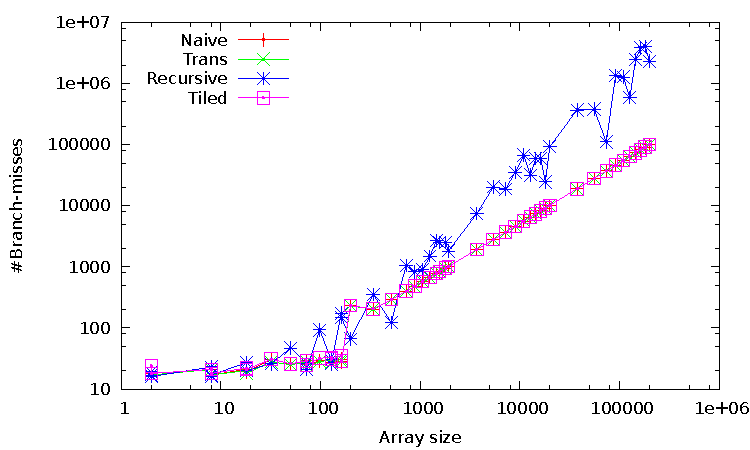
\includegraphics[width=\textwidth]{./Figures/Project2a/Branch_misses.pdf}
		\rule{35em}{0.5pt}
	\caption[Branch misses]{
	Bla bla bla.
	}
	\label{fig:Branch_misses}
\end{figure}


\begin{figure}[htbp]
	\centering
		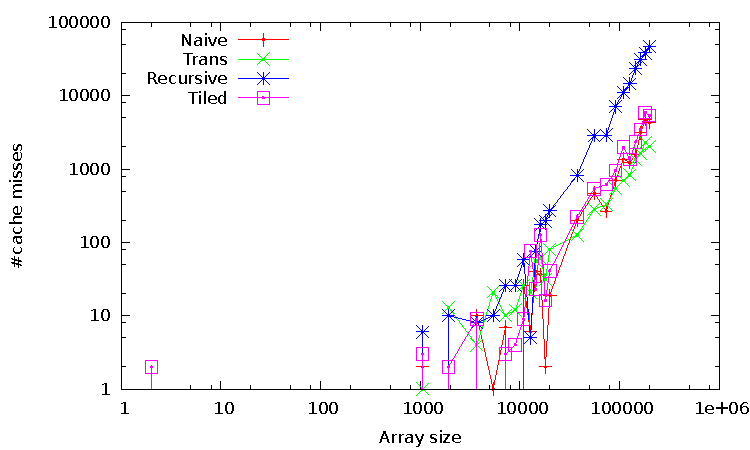
\includegraphics[width=\textwidth]{./Figures/Project2a/Cache_misses.pdf}
		\rule{35em}{0.5pt}
	\caption[Cache misses]{
	Bla bla bla.
	}
	\label{fig:Cache_misses}
\end{figure}



\begin{figure}[htbp]
	\centering
		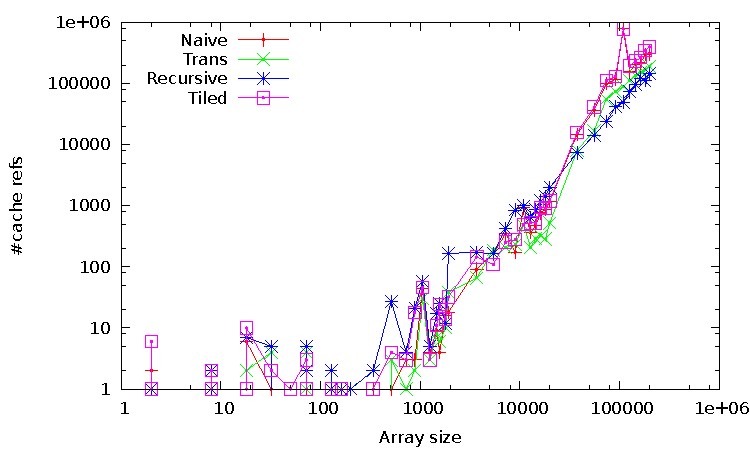
\includegraphics[width=\textwidth]{./Figures/Project2a/Cache_refs.pdf}
		\rule{35em}{0.5pt}
	\caption[Cache refs]{
	Bla bla bla.
	}
	\label{fig:Cache_refs}
\end{figure}



\begin{figure}[htbp]
	\centering
		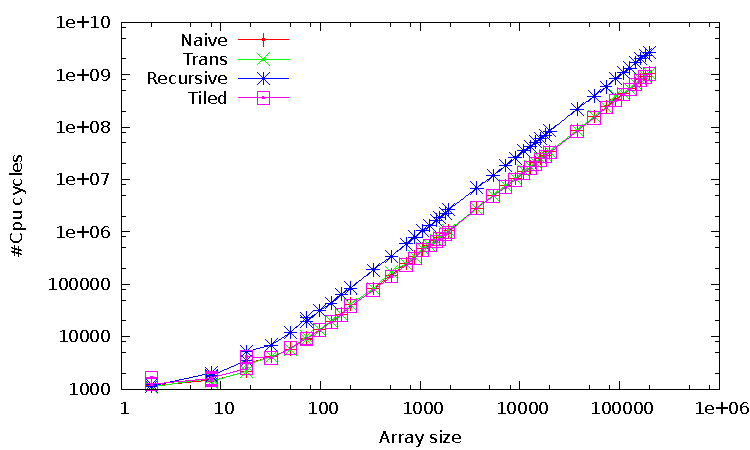
\includegraphics[width=\textwidth]{./Figures/Project2a/Cpu_cycles.pdf}
		\rule{35em}{0.5pt}
	\caption[CPU cycles]{
	Bla bla bla.
	}
	\label{fig:Cpu_cycles}
\end{figure}


\begin{figure}[htbp]
	\centering
		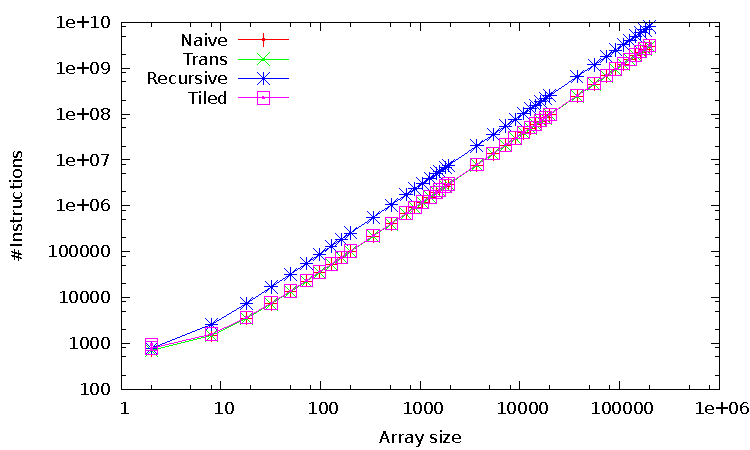
\includegraphics[width=\textwidth]{./Figures/Project2a/Instructions.pdf}
		\rule{35em}{0.5pt}
	\caption[Instructions]{
	Bla bla bla.
	}
	\label{fig:Instructions}
\end{figure}
